\documentclass{beamer}
\usepackage[utf8]{inputenc}
\usepackage[brazil]{babel}
\usepackage[T1]{fontenc}
\usetikzlibrary{positioning}
\usepackage{twemojis}

% Preamble
\usetheme{Madrid} % Set beamer theme

% slides set to always display the current section name at their header
\newcommand{\slide}[2]{
	\begin{frame}{\insertsection}
		\framesubtitle{#1}
		#2
	\end{frame}
} 

% Custom footer displaying solely the slide count
\setbeamertemplate{footline}{%
  \begin{beamercolorbox}[wd=\paperwidth,ht=2.25ex,dp=1ex,right]{footline}%
    \hfill%
    \usebeamerfont{page number in head/foot}%
    \insertframenumber/\inserttotalframenumber%
    \kern1em\vskip2pt%
  \end{beamercolorbox}%
}
\setbeamertemplate{navigation symbols}{} % Remove navigation icons

\title[SCC0217]{Ambientes de Execução em Compiladores}
\subtitle{Disciplina SCC0217 (2025) — Grupo 1, Turma 2}
\author{
	\begin{tabular}{ll}
		\hline
		\textbf{Nome} & \textbf{NUSP} \\
		\hline
		Guilherme de Abreu Barreto & 12543033 \\
		Hélio Nogueira Cardoso & 10310227 \\
		Laura Fernandes Camargos & 13692334 \\
		Sandy da Costa Dutra & 12544570 \\
		Theo da Mota dos Santos & 10691331 \\
	\end{tabular}
}
\institute{
	Instituto de Ciências Matemáticas e de Computação\\
	Universidade de São Paulo, ICMC - USP
}
\date{\today}

% Begin document
\begin{document}

\begin{frame}
	\titlepage
\end{frame}


\section{Introdução}

\slide{O que é um ambiente de execução?}{
	\begin{itemize}
		\item Estrutura de registros de memória do computador-alvo
		      \pause
		\item Responsável por:
		      \begin{itemize}
			      \item Gerenciamento de memória (alocação/liberamento)
			            \pause
			      \item Manutenção das informações necessárias para execução
			            \pause
			      \item Controle do fluxo de chamadas de funções/procedimentos
		      \end{itemize}
	\end{itemize}
}

\slide{Principais categorias}{
	\begin{itemize}
		\item Baseado em pilhas
		      \begin{itemize}
			      \item C/C++, Pascal
		      \end{itemize}
		      \pause
		\item Totalmente estático
		      \begin{itemize}
			      \item FORTRAN77
		      \end{itemize}
		      \pause
		\item Totalmente dinâmico
		      \begin{itemize}
			      \item Linguagens funcionais como Lisp e Haskell
		      \end{itemize}

	\end{itemize}
}

\section{Ambientes Baseados em Pilhas}

\slide{Aspectos Gerais}{
	\begin{itemize}
		\item Estrutura composta por pilha, heap e espaço livre
		      \pause
		\item Armazenamento de registros de ativação de procedimentos
		      \pause
		\item Controle de fluxo por registradores
	\end{itemize}
}

\slide{Regiões de Memória}{

	\begin{itemize}
		\item Área de Código: Instruções, valores constantes e variáveis globais. Todas as informações para as quais o endereço de memória é conhecido e estático.
		      \pause
		\item Área de Dados: Todos os demais dados cujo endereço de memória muda conforme cada contexto de execução do programa.
	\end{itemize}

	\vspace{0.5cm}

	\centering
	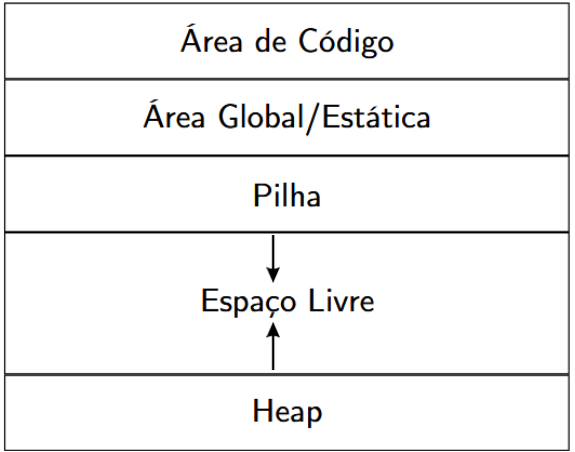
\includegraphics[width=0.45\textwidth]{images/memoria_pilha.png}
}

\slide{Área de dados}{

	\begin{itemize}
		\item Área de Pilha: dados cuja alocação ocorre na forma LIFO.
		\item Área de Heap: onde são armazenados dinamicamente quaisquer outros dados que não seguem essa ordenação.
		\item Espaço Livre: área de memória disponível para alocação tanto pela pilha quanto pelo heap.
	\end{itemize}

	\vspace{0.5cm}

	\centering
	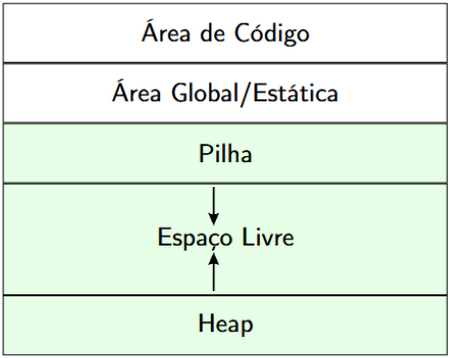
\includegraphics[width=0.45\textwidth]{images/memoria_verde.png}
}

\slide{Registro de ativação}{
	\begin{itemize}
		\item Durante a execução do programa, cada chamada de função cria na pilha um registro de ativação.
		\item Um registro de ativação é composto por, no mínimo, espaço para os seguintes elementos:
		      \begin{itemize}
			      \item Argumentos (ou parâmetros)
			      \item Dados locais
			      \item Endereço de retorno
		      \end{itemize}
	\end{itemize}
}

\slide{Registradores}{
	\begin{itemize}
		\item Armazenam valores pertinentes ao momento atual da execução de um programa
		\item Registradores de uso específico para acompanhar a execução:
		      \begin{itemize}
			      \item Contador de programa (pc)
			      \item Ponteiro de pilha(sp)
			      \item Ponteiro de quadros (fp)
			      \item Ponteiro de argumentos (ap)
		      \end{itemize}
		\item Para que servem?
	\end{itemize}
}

\slide{Exemplo de chamada e retorno de função}{
	\centering
	\scriptsize
	\begin{tikzpicture}[
			frame/.style={draw, rectangle, minimum width=4cm, minimum height=1.2cm, align=left},
			arrow/.style={->, >=stealth, thick},
			txt/.style={align=left},
			>=stealth
		]

		\node[frame, fill=blue!10] (main) at (0,0) {
			\textbf{main()}\\\hline
			FP $\rightarrow$ Variáveis locais\\
			Endereço de retorno (sp)
		};

		\node[frame, fill=green!10, below=0.3cm of main] (func1) {
			\textbf{func1()}\\\hline
			FP $\rightarrow$ Parâmetros (a, b)\\
			Variáveis locais\\
			Endereço de retorno (main)
		};

		\node[frame, fill=red!10, below=0.3cm of func1] (func2) {
			\textbf{func2()}\\\hline
			FP $\rightarrow$ Parâmetros (x)\\
			Variáveis locais\\
			Endereço de retorno (func1)
		};

		% Ponteiros SP e FP
		\draw[arrow] ([xshift=-1.8cm]main.west) -- node[left] {sp} ([xshift=-1.8cm]func2.south west);

		% Chamada de funções
		\node[txt, above left=0.5cm and 1cm of main] (call1) {\texttt{func1(a, b)}};
		\draw[arrow] (call1) -- (main.west);

		\node[txt, right=1.2cm of func1] (call2) {\texttt{func2(x)}};
		\draw[arrow] (call2) -- (func1.east);

		% Retorno
		\node[txt, below right=0.5cm and 1cm of func2] (return) {\texttt{return y}};
		\draw[arrow] (func2.south) -- (return);

		%
		%    1. Empilha registro de ativação\\
		%    2. Atualiza SP e FP\\[0.2cm]
		%    \textbf{Retorno:}\\
		%    1. Restaura FP anterior\\
		%    2. Ajusta SP\\
		%    3. Retoma execução

	\end{tikzpicture}
}

\begin{frame}{Sequências de Ativação e Retorno}
	\begin{itemize}
		\item \textbf{Sequência de Ativação}:
		      \begin{itemize}
			      \item Computação e armazenamento de argumentos.
			      \item Armazenamento de FP e endereço de retorno.
			      \item Atualização de PC.
		      \end{itemize}
		\item \textbf{Sequência de Retorno}:
		      \begin{itemize}
			      \item Restauração de FP e PC.
		      \end{itemize}
	\end{itemize}
\end{frame}

\begin{frame}{Dados de Comprimento Variável}
	\begin{itemize}
		\item \textbf{Exemplo}: Funções com argumentos variáveis (e.g., Ada).
		\item \textbf{Organização}: Armazenamento de tamanho e quantidade na pilha.
	\end{itemize}
\end{frame}

\begin{frame}{Gerenciamento de Heap}
	\begin{itemize}
		\item \textbf{Alocação} (malloc): Busca bloco livre e ajusta ponteiros.
		\item \textbf{Liberação} (free): Marca bloco como disponível.
	\end{itemize}
\end{frame}

\begin{frame}{Ambientes Sem Procedimentos Locais}
	\begin{itemize}
		\item \textbf{Exemplo}: Linguagem C (funções globais).
		\item \textbf{Registradores}: FP e FP old.
	\end{itemize}
\end{frame}

\begin{frame}{Ambientes Com Procedimentos Locais}
	\begin{itemize}
		\item \textbf{Exemplo}: Pascal, Lua (funções aninhadas).
		\item \textbf{Vinculação de Acesso}: Endereço da função declaradora.
	\end{itemize}
\end{frame}

\begin{frame}{Ambientes Com Parâmetros de Procedimentos}
	\begin{itemize}
		\item \textbf{Exemplo}: Passagem de funções como argumentos (Pascal, Lua).
		\item \textbf{Ponteiros}: IP (Instruction Pointer) e EP (Environment Pointer).
	\end{itemize}
\end{frame}

\section{Ambientes de execução totalmente estáticos}

\begin{frame}{Ambientes Totalmente Estáticos}
	\begin{itemize}
		\item \textbf{Características}:
		      \begin{itemize}
			      \item Dados em posições fixas.
			      \item Sem ponteiros, alocação dinâmica ou recursão.
		      \end{itemize}
		\item \textbf{Exemplo}: FORTRAN77.
	\end{itemize}
\end{frame}

\section{Ambientes de execução totalmente dinâmicos}

\begin{frame}{Ambientes de Execução Totalmente Dinâmicos}
	\begin{itemize}
		\item \textbf{Características}:
		      \begin{itemize}
			      \item Uso exclusivo do heap.
			      \item Referências pendentes evitadas com coleta de lixo.
		      \end{itemize}
		\item \textbf{Exemplo}: Haskell, LISP.
	\end{itemize}
\end{frame}

\slide{Coleta de Lixo (\textit{garbage collection})}{
	Abordagem de gerenciamento de memória caraterística de ambientes de
	execução totalmente dinâmicos. \pause Seu uso requer:
	\begin{itemize}
		\item o acompanhamento das referências durante a execução;
		      \pause
		\item capacidade para encontrar e liberar porções da memória já inacessíveis em instantes arbitrários durante a execução.
	\end{itemize}
}

\slide{Marcar e correr (\textit{mark and sweep})}{
	Principal algoritmo de coleta de lixo. \pause Neste, a cada sequência de ativação, ocorrem duas passadas pelo \textit{heap}.

	\begin{itemize}
		\item Na primeira passada:
		      \pause
		      \begin{itemize}
			      \item Percorre-se todos os ponteiros ao heap recursivamente;
			            \pause
			      \item Marca-se cada bloco acessado desta forma com um bit de validação, indicando que este é "alcançável".
		      \end{itemize}
		\item Na segunda passada:
		      \pause
		      \begin{itemize}
			      \item Percorre-se o \textit{heap} linearmente, liberando a memória de todos os blocos que não foram marcados como sendo alcançáveis.
			            \pause

			      \item O novo registro de ativação é armazenado no primeiro
			            bloco de memória a satisfazer seu requerimento de memória,
			            \textbf{se este houver}.

		      \end{itemize}
	\end{itemize}
}

\slide{Marcar e correr (\textit{mark and sweep})}{
	Nos casos em que o requerimento de memória não é satisfeito, ocorre
	compactação.
}

\slide{Marcar e correr (\textit{mark and sweep})}{
	São contrapontos ao uso de coleta de lixo:
	\pause
	\begin{enumerate}
		\item Requer memória adicional para marcar blocos alcançáveis.
		      \pause
		\item Requer pelo menos duas passadas pela memória \textit{heap} a cada sequência de
		      ativação
	\end{enumerate}
	\pause
	Mas existem otimizações que mitigam estas limitações.
}

\slide{Otimizações}{
	\textbf{Parar e copiar}. Nesta, o heap é dividido em duas regiões de tamanho
	variável: \pause a primeira possui blocos ocupados e a segunda um
	bloco contíguo de memória livre. \pause A cada sequência de ativação,

	\begin{itemize}
		\item O novo registro de ativação é alocado no endereço do bloco livre;
		      \pause
		\item Realiza-se uma única passada
		      \pause
		\item Trocam-se os papéis
	\end{itemize}
}

\slide{Otimizações}{
	\textbf{Coleta de lixo generativa}. Nesta, uma terceira região de memória é
	adicionada ao heap para dados ``permanentes''.
}

\section{Considerações finais}


\slide{}{
	Abarcamos os três principais ambientes de execução que fundamentam a uma
	variedade de linguagens programação. \pause Cada qual destaca a adaptabilidade das linguagens de programação às diferentes necessidades computacionais.

	\vspace{2cm}
	\pause\centering
	Obrigado pela audiência! \twemoji{wave}
}

\end{document}
